\chapter{General Matching and Edmonds Blossom Algorithm}

A matching in a graph is a set of edges, no two of which share a vertex. Every reader of the
previous two chapters knows how to find a maximum matching in a \emph{bipartite} graph: orient the
edges, push flow, or chase augmenting paths along the two-sided structure. The natural question is
whether the same machinery works on an arbitrary graph. It very nearly does. The augmenting-path
idea survives untouched; what breaks is the bookkeeping that finds those paths. A single odd cycle
is enough to fool the breadth-first search that worked so cleanly on bipartite graphs, and repairing
that failure is the entire content of this chapter.

The repair is Jack Edmonds' 1965 \emph{blossom} algorithm. It is a landmark in
combinatorial optimization: it resolved a problem that had resisted efficient solution for decades,
and its introductory paper (``Paths, Trees, and Flowers'') formalized polynomial-time solvability as
the theoretical benchmark for algorithmic efficiency. We build the algorithm from the augmenting-path
skeleton, examine precisely where odd cycles cause parity ambiguities, introduce the contraction
operation that resolves them, prove that contraction preserves augmenting paths, and trace the execution
on a concrete example. We close with the Tutte--Berge formula---the min-max duality theorem that certifies
the maximum matching size---and the primal--dual weighted generalization.

\chapterline

\section{Matchings, Augmenting Paths, and Berge's Theorem}

Fix an undirected graph $\Gph=(V,E)$ with $n=\abs{V}$ and $m=\abs{E}$. We make no bipartiteness
assumption.

\begin{definition}[Matching]
\label{ch17:def-matching}
A \emph{matching} $M\subseteq E$ is a set of edges with no shared endpoints. A vertex incident to an
edge of $M$ is \emph{matched} (or \emph{covered}); otherwise it is \emph{free} (or
\emph{exposed}). $M$ is \emph{maximum} if no matching has more edges, and \emph{perfect} if it covers
every vertex.
\end{definition}

Maximum and \emph{maximal} are different words. A maximal matching is one you cannot enlarge by adding
a single edge; a maximum matching is globally largest. A path graph $a\!-\!b\!-\!c\!-\!d$ has the
maximal matching $\set{bc}$ of size one, but the maximum matching $\set{ab,cd}$ has size two. The
greedy ``add any edge that fits'' procedure gives a maximal matching, and it can be off by a factor of
two. We want maximum.

\begin{intuitionbox}
Think of a matching as a set of committed monogamous pairs. To grow it, we want to find a free
person, lead a chain of swaps through the currently-paired people, and arrive at another free person.
If such a chain exists, we can re-pair everybody along it and net one extra couple. That chain is an
augmenting path, and the whole theory of matching is the theory of finding one (or proving none
exists).
\end{intuitionbox}

\begin{definition}[Alternating and augmenting paths]
\label{ch17:def-augpath}
Given a matching $M$, a path is \emph{$M$-alternating} if its edges alternate between $E\setminus M$
and $M$. An alternating path is \emph{$M$-augmenting} if it is \emph{simple} and both endpoints are
free.
\end{definition}

An augmenting path necessarily has odd length: it starts and ends with a non-matching edge, so the
pattern is $\notin M,\ \in M,\ \notin M,\dots,\notin M$. If $P$ is augmenting, flipping every edge of
$P$ (matched becomes unmatched and vice versa) produces a matching $M\oplus P$ -- the symmetric
difference -- with exactly one more edge. The two endpoints become matched and every interior vertex
stays matched, just to a different partner.

\begin{theorem}[Berge, 1957]
\label{ch17:thm-berge}
A matching $M$ is maximum if and only if $\Gph$ contains no $M$-augmenting path.
\end{theorem}

\begin{whybox}
The forward direction is immediate: an augmenting path lets us build a strictly larger matching, so a
maximum $M$ admits none. The reverse direction is the workhorse, and its proof is a structural fact
about the symmetric difference of two matchings that we will reuse constantly.
\end{whybox}

\begin{proof}
($\Rightarrow$) If $P$ is $M$-augmenting then $\abs{M\oplus P}=\abs{M}+1$, so $M$ is not maximum.
Contrapositive gives the claim.

($\Leftarrow$) Suppose $M$ is not maximum; let $M^{\star}$ be a larger matching, so
$\abs{M^{\star}}>\abs{M}$. Consider the edge set $H=M\oplus M^{\star}$ and the subgraph it spans.
Every vertex has degree at most one in $M$ and at most one in $M^{\star}$, hence degree at most two in
$H$. A graph of maximum degree two is a disjoint union of simple paths and cycles. Along any such
component the edges alternate between $M$ and $M^{\star}$ (two $M$-edges at a vertex would violate the
matching property, likewise two $M^{\star}$-edges). Therefore every cycle has even length and
contains equally many $M$- and $M^{\star}$-edges. Since $M^{\star}$ contributes more edges overall
than $M$, some path component must contain more $M^{\star}$-edges than $M$-edges. Such a path begins
and ends with an $M^{\star}$-edge; its endpoints are thus free in $M$ (they are covered in
$M^{\star}$, not in $M$). That path is alternating with respect to $M$ and has both ends free: an
$M$-augmenting path. Contradiction.
\end{proof}

Berge's theorem reduces ``find a maximum matching'' to the loop:

\begin{center}
\emph{while an augmenting path exists, find one and flip it.}
\end{center}

Each flip raises $\abs{M}$ by one, so the loop runs at most $n/2$ times. Everything now hinges on a
single subroutine: \textsc{FindAugmentingPath}. In a bipartite graph that subroutine is an ordinary
search. In a general graph it is where the trouble lives.

\begin{historybox}
Berge's lemma (Claude Berge, 1957) predates Edmonds and applies to any graph. For bipartite graphs
K\H{o}nig (1931) and the Hungarian method already exploited augmenting paths. The open problem for the
next eight years was purely algorithmic: can you \emph{find} an augmenting path in a non-bipartite
graph in polynomial time? Edmonds answered yes in 1965 and, in the same breath, argued that
``polynomial'' is the right notion of a good algorithm -- a thesis that organized the whole field of
complexity theory that followed.
\end{historybox}

\section{Why Odd Cycles Break the Bipartite Search}

To find an augmenting path we grow a search tree from a free vertex, alternating as we go. Root the
tree at a free vertex $r$. Label $r$ \emph{even} (an even number of edges from the root). From an
even vertex we step along a \emph{non-matching} edge to a neighbour and label it \emph{odd}; from an
odd vertex we step along the unique \emph{matching} edge to its partner and label it \emph{even}. An
even-labelled vertex is reached by an even-length alternating path from $r$, so if we ever reach a
\emph{free} vertex with an even label we have closed an augmenting path. This is the engine of every
matching algorithm; in the literature the search tree is called an \emph{alternating tree}.

\begin{center}
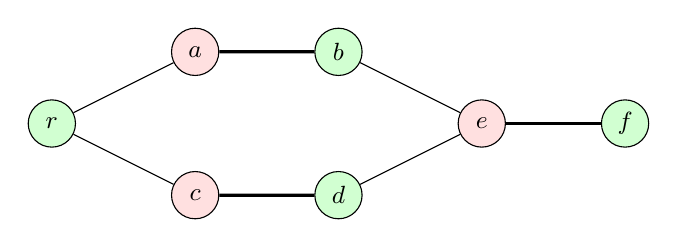
\begin{tikzpicture}[every node/.style={circle,draw,minimum size=6mm,inner sep=0pt,font=\small},
  matched/.style={very thick}, scale=1.3]
\node[fill=green!18] (r) at (0,0) {$r$};
\node[fill=red!12] (a) at (1.4,0.7) {$a$};
\node[fill=green!18] (b) at (2.8,0.7) {$b$};
\node[fill=red!12] (c) at (1.4,-0.7) {$c$};
\node[fill=green!18] (d) at (2.8,-0.7) {$d$};
\node[fill=red!12] (e) at (4.2,0) {$e$};
\node[fill=green!18] (f) at (5.6,0) {$f$};
\draw (r)--(a); \draw[matched] (a)--(b);
\draw (r)--(c); \draw[matched] (c)--(d);
\draw (b)--(e); \draw (d)--(e); \draw[matched] (e)--(f);
\end{tikzpicture}
\end{center}

Green discs are even vertices, red discs are odd, thick edges are matched. So far the tree behaves
itself: from the root $r$ we reached $b$ and $d$ (even) along matched edges through $a,c$ (odd), and
the search would continue from $b$ and $d$.

Now look at what happens at $e$. From even $b$ we step along the non-matching edge $b\!-\!e$ and want
to call $e$ odd. But from even $d$ we also reach $e$ along the non-matching edge $d\!-\!e$, and that
call also wants $e$ odd. The two even vertices $b$ and $d$ are joined (through $e$) by an even-length
alternating path inside the tree plus the edges $be$ and $de$ -- together with $e$ they form an odd
closed walk $b\!-\!e\!-\!d\!-\dots-\!b$. The vertex $e$ can be labelled \emph{both} even and
odd depending on which root-path you take to it. That ambiguity is the whole difficulty.

\begin{intuitionbox}
In a bipartite graph this never happens. Bipartite graphs are exactly the graphs with no odd cycle,
so the BFS layering into even and odd is consistent -- a vertex's parity is determined by the graph,
not by the path you took. The moment an \emph{odd} cycle appears, a vertex can be reached by both an
even and an odd alternating path, and the clean even/odd labelling collapses. That is the whole
difficulty of general matching in one sentence.
\end{intuitionbox}

The canonical trap that illustrates this ambiguity is a five-cycle carrying a near-perfect matching, with one free vertex on the rim and a free pendant attached to it, as shown in Figure~\ref{ch17:fig-parity-trap}.

\begin{figure}[H]
\centering
\begin{tikzpicture}[
  every node/.style={circle,draw=black!80,thick,minimum size=6.5mm,inner sep=0pt,font=\small},
  even/.style={fill=targetgreen!20,draw=targetgreen!80},
  odd/.style={fill=trapred!20,draw=trapred!80},
  ambi/.style={fill=quotientorange!25,draw=quotientorange!80,very thick},
  matched/.style={line width=2pt,trapred},
  unmatched/.style={line width=0.8pt,edgegray}
]
\node[even] (r) at (-1.8,0) {$r$};
\node[odd]  (v1) at (-0.2,0) {$1$};
\node[ambi] (v2) at (0.9,0.95) {$2$};
\node[ambi] (v3) at (2.1,0.55) {$3$};
\node[ambi] (v4) at (2.1,-0.55) {$4$};
\node[ambi] (v5) at (0.9,-0.95) {$5$};

\draw[unmatched] (r) -- (v1);
\draw[unmatched] (v1) -- (v2);
\draw[matched]   (v2) -- (v3) node[midway,above=2pt,sloped,font=\scriptsize,trapred] {$\in M$};
\draw[unmatched] (v3) -- (v4);
\draw[matched]   (v4) -- (v5) node[midway,below=2pt,sloped,font=\scriptsize,trapred] {$\in M$};
\draw[unmatched] (v5) -- (v1);

\node[draw=none,fill=none,font=\footnotesize,align=center] at (1.1,-1.6)
  {Rim vertices $2,3,4,5$ possess \emph{both} even and odd parity\\
   depending on whether the cycle is traversed clockwise or counterclockwise};
\end{tikzpicture}
\caption{The parity ambiguity on an odd cycle. Starting an alternating
breadth-first tree from free root $r$, vertex $1$ is reached via unmatched edge $r1$
and labelled odd. Traversing clockwise, $2$ is even and $3$ is odd. But traversing
counterclockwise, $5$ is even and $4$ is odd. Because the cycle length is odd ($5$),
each rim vertex can be reached by both an even-length and an odd-length alternating
path, defeating standard bipartite BFS level assignments.}
\label{ch17:fig-parity-trap}
\end{figure}

Here $M=\set{23,45}$, with vertices $1$ and $r$ free. Grow the tree from $r$: $r$ is even, $1$ is odd
via the stem $r1$, but $1$ is also reachable as an \emph{even} vertex by walking the cycle: $1\,2\,3$
makes $1$ even, $2$ odd, $3$ even; and $1\,5\,4$ makes $1$ even, $5$ odd, $4$ even. The five-cycle
relabels its rim vertices with both parities. A naive search that commits to the first label it
assigns will either loop or miss the augmenting path that runs through the cycle. The cure is to
recognize the odd cycle and collapse it.

\section{Blossoms, Stems, and Contraction}

\begin{definition}[Blossom]
\label{ch17:def-blossom}
Let $M$ be a matching and let the alternating-tree search be in progress. A \emph{blossom} is an
odd-length cycle $C=v_0 v_1 \cdots v_{2k} v_0$ with exactly $k$ matched edges, in which the vertex
$v_0$ (the \emph{base}) is the unique vertex not matched \emph{inside} $C$. Equivalently, $C$ has
$2k+1$ edges, $k$ of them in $M$, and every vertex except the base is matched along $C$.
\end{definition}

The base $v_0$ is either free or matched by an edge leaving $C$ (the matched edge that connects the
blossom to the rest of the tree). The alternating path from the root $r$ down to the base is the
\emph{stem}; it has even length and ends with a matched edge into $v_0$ (or is empty if $v_0=r$).
Stem plus blossom is a \emph{flower}.

\begin{center}
\begin{tikzpicture}[every node/.style={circle,draw,minimum size=6mm,inner sep=0pt,font=\small},
  matched/.style={very thick}, scale=1.35]
\node[fill=green!18] (r) at (-3.2,0) {$r$};
\node[fill=red!12]   (s) at (-2.0,0) {$s$};
\node[fill=green!18] (b) at (-0.8,0) {$v_0$};
\node[fill=red!12]   (v1) at (0.3,0.95) {$v_1$};
\node[fill=green!18] (v2) at (1.5,0.8) {$v_2$};
\node[fill=red!12]   (v3) at (2.0,-0.2) {$v_3$};
\node[fill=green!18] (v4) at (1.0,-0.95) {$v_4$};
\draw (r)--(s);
\draw[matched] (s)--(b);
\draw (b)--(v1);
\draw[matched] (v1)--(v2);
\draw (v2)--(v3);
\draw[matched] (v3)--(v4);
\draw (v4)--(b);
\draw[decorate,decoration={brace,amplitude=5pt},red!55!black]
  (-3.3,-0.55) -- (-0.7,-0.55) node[midway,below=4pt,draw=none,fill=none,font=\footnotesize]{stem (even)};
\draw[decorate,decoration={brace,amplitude=5pt,mirror},structurepurple]
  (-0.6,1.2) -- (2.2,1.2) node[midway,above=4pt,draw=none,fill=none,font=\footnotesize]{blossom $C$};
\end{tikzpicture}
\end{center}

A blossom here is the five-cycle $v_0 v_1 v_2 v_3 v_4 v_0$ with base $v_0$, matched edges $v_1v_2$ and
$v_3v_4$, and base reached from $r$ by the stem $r\!-\!s\!-\!v_0$ (matched edge $s v_0$).

The structural fact that makes everything work is that \emph{every} vertex of a blossom is reachable
from the base by an alternating path of \emph{even} length that ends with a non-matching edge. Because
you can go around the odd cycle in two directions, each non-base vertex enjoys both parities. That is
precisely the ambiguity that broke the search; inside a blossom it is a feature, because it means we
can splice into the cycle from either side.

\begin{lemma}[Even reachability inside a blossom]
\label{ch17:lem-blossom-even}
Let $C$ be a blossom with base $v_0$. For every vertex $u\in C$ there is an $M$-alternating path
inside $C$ from $v_0$ to $u$ of even length (possibly length $0$ for $u=v_0$) whose first edge (the
one leaving the base) is unmatched and whose final edge (the one entering $u$) is matched whenever
$u\neq v_0$.
\end{lemma}

\begin{proof}
Index the cycle $v_0 v_1 \cdots v_{2k} v_0$ so that the matched edges are
$v_1 v_2, v_3 v_4, \dots, v_{2k-1} v_{2k}$. Going \emph{clockwise} $v_0 v_1 v_2 \cdots v_i$ the edges
alternate starting with the unmatched edge $v_0 v_1$; this path has length $i$. Going
\emph{counterclockwise} $v_0 v_{2k} v_{2k-1}\cdots v_i$ starts with the unmatched edge $v_0 v_{2k}$
and has length $2k+1-i$. The two lengths $i$ and $2k+1-i$ have opposite parities (their sum is the odd
number $2k+1$), so exactly one of the two routes reaches $v_i$ in an even number of steps. Take that
route; by construction it starts at the base with an unmatched edge and, being alternating of even
length, ends with a matched edge into $v_i$ (an even-length path that opens with an unmatched edge
closes with a matched one).
\end{proof}

\subsection{Contraction}

Edmonds' insight was that when the search discovers a blossom $C$, it should \emph{contract} it. Replace all vertices of
$C$ by a single super-vertex $B$. Every edge from a vertex outside $C$ to a vertex inside $C$ now
attaches to $B$ (parallel edges are allowed and harmless); edges inside $C$ vanish. Call the smaller graph
$\Gph/B$ and let $M/B$ be the matching with the blossom's internal edges removed -- the $k$ internal
matched edges disappear, while the base's external matched edge (if any) survives and now matches the
super-vertex $B$. The super-vertex is matched iff the base was matched, and it inherits the base's
even label in the tree.

Figure~\ref{ch17:fig-blossom-shrink-lift} illustrates this entire contraction and path lifting lifecycle.

\begin{figure}[H]
\centering
\begin{tikzpicture}[
  every node/.style={font=\small},
  ev/.style={circle,draw=targetgreen!80,thick,fill=green!15,minimum size=6mm,inner sep=0pt},
  od/.style={circle,draw=trapred!80,thick,fill=red!15,minimum size=6mm,inner sep=0pt},
  bv/.style={circle,draw=structurepurple,very thick,fill=structurepurple!15,minimum size=8mm,inner sep=0pt},
  mat/.style={line width=1.8pt,trapred},
  unm/.style={line width=0.8pt,edgegray},
  aug/.style={line width=2pt,quotientorange,dashed},
  arrowaug/.style={-{Stealth[length=2.5mm]},quotientorange,line width=1.8pt}
]
% Panel (a): The Original Flower (Stem + Blossom)
\begin{scope}
  \node[font=\footnotesize\bfseries,align=center] at (1.8,2.7) {\textbf{(a)} The Flower ($G, M$)};

  \node[ev] (r)  at (-0.6,0.8) {$r$};
  \node[od] (s)  at (0.4,0.8)  {$s$};
  \node[ev] (b)  at (1.4,0.8)  {$v_0$};

  \node[od] (v1) at (2.2,1.6)  {$v_1$};
  \node[ev] (v2) at (3.2,1.3)  {$v_2$};
  \node[ev] (v3) at (3.2,0.3)  {$v_3$};
  \node[od] (v4) at (2.2,0.0)  {$v_4$};

  \node[ev] (w)  at (4.2,0.3)  {$w$};

  \draw[unm] (r) -- (s);
  \draw[mat] (s) -- (b) node[pos=0.5,above=1pt,font=\scriptsize,trapred] {$\in M$};

  \draw[unm] (b) -- (v1);
  \draw[mat] (v1) -- (v2) node[pos=0.5,above=1pt,font=\scriptsize,trapred] {$\in M$};
  \draw[unm] (v2) -- (v3);
  \draw[mat] (v3) -- (v4) node[pos=0.5,below=1pt,font=\scriptsize,trapred] {$\in M$};
  \draw[unm] (v4) -- (b);

  \draw[unm] (v3) -- (w) node[pos=0.5,above=1pt,font=\scriptsize,edgegray] {free};

  \draw[draw=structurepurple!60,dashed,rounded corners=6pt] (1.1,-0.3) rectangle (3.5,1.9);
  \node[structurepurple,font=\scriptsize\bfseries] at (2.3,2.1) {Blossom $B$};

  \node[font=\footnotesize,align=center] at (1.8,-0.9)
    {Stem $r{-}s{-}v_0$ connects to\\blossom base $v_0$; $w$ is free};
\end{scope}

% Panel (b): Contraction to Pseudo-Vertex B
\begin{scope}[xshift=5.3cm]
  \node[font=\footnotesize\bfseries,align=center] at (1.7,2.7) {\textbf{(b)} Contracted Graph ($G/B$)};

  \node[ev] (br) at (0.0,0.8) {$r$};
  \node[od] (bs) at (1.0,0.8) {$s$};
  \node[bv] (bB) at (2.2,0.8) {$B$};
  \node[ev] (bw) at (3.4,0.8) {$w$};

  \draw[unm] (br) -- (bs);
  \draw[mat] (bs) -- (bB) node[pos=0.5,above=1pt,font=\scriptsize,trapred] {$\in M/B$};
  \draw[unm] (bB) -- (bw) node[pos=0.5,above=1pt,font=\scriptsize,edgegray] {unmatched};

  % Augmenting path highlight in G/B
  \draw[aug] (br) -- (bs) -- (bB) -- (bw);
  \node[quotientorange,font=\scriptsize\bfseries] at (1.7,0.1) {Augmenting: $r \rightsquigarrow w$};

  \node[font=\footnotesize,align=center] at (1.7,-0.9)
    {Blossom shrunk to super-vertex $B$;\\
     augmenting path easily found};
\end{scope}

% Panel (c): Path Lifting / Unrolling
\begin{scope}[xshift=9.8cm]
  \node[font=\footnotesize\bfseries,align=center] at (1.8,2.7) {\textbf{(c)} Path Lifting in $G$};

  \node[ev] (cr)  at (-0.6,0.8) {$r$};
  \node[od] (cs)  at (0.4,0.8)  {$s$};
  \node[ev] (cb)  at (1.4,0.8)  {$v_0$};

  \node[od] (cv1) at (2.2,1.6)  {$v_1$};
  \node[ev] (cv2) at (3.2,1.3)  {$v_2$};
  \node[ev] (cv3) at (3.2,0.3)  {$v_3$};
  \node[od] (cv4) at (2.2,0.0)  {$v_4$};

  \node[ev] (cw)  at (4.2,0.3)  {$w$};

  % Background unselected edges
  \draw[edgegray!35] (cb) -- (cv1);
  \draw[edgegray!35] (cv1) -- (cv2);
  \draw[edgegray!35] (cv2) -- (cv3);

  % Lifted augmenting path
  \draw[arrowaug] (cw) -- (cv3);
  \draw[arrowaug] (cv3) -- (cv4);
  \draw[arrowaug] (cv4) -- (cb);
  \draw[arrowaug] (cb) -- (cs);
  \draw[arrowaug] (cs) -- (cr);

  \node[quotientorange,font=\scriptsize\bfseries,align=center] at (2.4,1.2) {Even arc\\$v_3 \to v_4 \to v_0$};

  \node[font=\footnotesize,align=center] at (1.8,-0.9)
    {Unroll $B$ along even alternating\\
     internal arc $v_3{-}v_4{-}v_0$ to base};
\end{scope}
\end{tikzpicture}
\caption{The blossom contraction and path lifting lifecycle. (a)~A flower consists
of an alternating stem from free root $r$ to base $v_0$, and an odd cycle $B$ with
near-perfect matching. An external free vertex $w$ connects to $v_3$. (b)~Contracting
blossom $B$ into a single pseudo-vertex collapses all internal cycle edges. In the
reduced graph $\Gph/B$, the alternating search quickly identifies the augmenting path
$r - s - B - w$. (c)~Lifting the path back to $\Gph$: upon entering the blossom at
$v_3$, the path routes around the odd cycle via the even alternating path
$v_3 - v_4 - v_0$ guaranteed by Lemma~\ref{ch17:lem-blossom-even}, exiting cleanly
at base $v_0$ and continuing along the stem to free root $r$.}
\label{ch17:fig-blossom-shrink-lift}
\end{figure}

\begin{focusbox}
Contraction turns the odd cycle into a single even-labelled vertex. The labelling ambiguity that
broke the search is gone because there is no longer a cycle to walk two ways around. We run the
ordinary alternating search on the smaller graph; if it finds an augmenting path through $B$, we
\emph{expand} the blossom and re-route the path through whichever side of the cycle restores
alternation. Lemma~\ref{ch17:lem-blossom-even} is exactly what guarantees a valid re-route exists.
\end{focusbox}

The correctness of contraction is the heart of the algorithm.

\begin{theorem}[Blossom contraction is matching-preserving]
\label{ch17:thm-contract}
Let $C$ be a blossom for matching $M$ with the base reachable from a free root by an even alternating
stem. Then $\Gph$ has an $M$-augmenting path \emph{if and only if} $\Gph/C$ has an
$(M/C)$-augmenting path. Moreover an augmenting path in $\Gph/C$ lifts to one in $\Gph$ in linear
time.
\end{theorem}

\begin{whybox}
The slogan is: \emph{a blossom may as well be a single free-or-matched super-vertex.} Any augmenting
path can be made to enter and leave the blossom only at its base, and Lemma~\ref{ch17:lem-blossom-even}
fills in the missing arc inside the cycle. The proof handles the two directions separately; the lift
direction is the constructive one used by the implementation.
\end{whybox}

\begin{proof}
($\Leftarrow$, the lift) Let $P'$ be an $(M/C)$-augmenting path in $\Gph/C$. If $P'$ avoids the
super-vertex $c$, it is already an $M$-augmenting path in $\Gph$ (none of its edges or vertices were
touched by contraction). So suppose $P'$ passes through $c$. The base $v_0$ is matched in $M$ exactly
when $c$ is matched in $M/C$, so the matched edge of $P'$ at $c$ (if any) is the base's external
matched edge $e^{\star}=v_0 w$. Walk $P'$ from one free endpoint; let it reach $c$ along an edge
$x v_i$ that, before contraction, hit the blossom at the specific vertex $v_i$. There are two cases.

If $c$ is matched in $P'$, then $P'$ enters $c$ along the unmatched edge $xv_i$ and leaves along the
matched edge $e^{\star}=v_0 w$. Replace the visit to $c$ by $\dots x\,v_i \rightsquigarrow v_0\, w
\dots$, where $v_i \rightsquigarrow v_0$ is the even alternating path inside $C$ from $v_i$ to the base
given by Lemma~\ref{ch17:lem-blossom-even}, read backwards. Its first edge $x v_i$ is unmatched, the
internal path is alternating and of even length, then $e^{\star}$ continues as a matched edge.
Alternation holds throughout.

If $c$ is free in $P'$ (so $c$ is an endpoint of $P'$, since augmenting paths have free endpoints),
then $P'$ enters $c$ along an unmatched edge $x v_i$ and stops. Replace the endpoint $c$ by the even
internal path $v_i \rightsquigarrow v_0$; its far end $v_0$ is free in $M$ (the base is free because
$c$ was free), so the lifted path ends at a free vertex. Alternation again holds. Either way the
lifted path is simple (the internal arc visits distinct blossom vertices) and $M$-augmenting.

($\Rightarrow$) Suppose $\Gph$ has an $M$-augmenting path $P$. If $P$ misses $C$ entirely it survives
contraction. Otherwise let $P$ meet $C$. Among all augmenting paths choose one meeting $C$ in the
fewest vertices; standard surgery (replace any returning excursion by the shorter internal arc, again
via Lemma~\ref{ch17:lem-blossom-even}) shows $P$ can be taken to enter $C$, possibly traverse part of
it, and exit, with all of that collapsing to a single pass through the base. Contracting that pass to
the super-vertex $c$ yields an alternating path $P'$ in $\Gph/C$ whose endpoints are the (unchanged)
free endpoints of $P$, except that if an endpoint lay inside $C$ then the base was free and $c$ becomes
the free endpoint. In all cases $P'$ is $(M/C)$-augmenting. A counting view confirms it without the
surgery: a maximum matching of $\Gph$ uses exactly $k$ edges inside any factor-critical blossom that it
covers, so $\nu(\Gph)=\nu(\Gph/C)+k$ and likewise $\abs{M}=\abs{M/C}+k$; hence $\Gph$ has a larger
matching than $M$ iff $\Gph/C$ has a larger matching than $M/C$, which by Berge
(Theorem~\ref{ch17:thm-berge}) is the augmenting-path statement.
\end{proof}

\begin{trapbox}
A frequent bug is contracting a cycle that is \emph{not} a blossom -- for instance an even cycle, or
an odd cycle whose base is not reachable by an even stem. Theorem~\ref{ch17:thm-contract} needs
\emph{both} conditions: an odd cycle with a single base unmatched inside it, \emph{and} an even
alternating stem from a free root. Contracting an arbitrary odd cycle can destroy augmenting paths.
The search structure guarantees these conditions automatically: a blossom is detected only when two
even-labelled tree vertices are joined by a non-matching edge, and their lowest common ancestor in the
alternating tree is the base.
\end{trapbox}

\section{The Blossom Algorithm}

We now assemble the pieces. The outer loop is Berge's: repeatedly search for an augmenting path from
some free vertex and flip it. The inner search grows an alternating tree, contracting blossoms as it
meets them, until it either finds an augmenting path (success) or exhausts the tree (this free vertex
can never be matched in a larger matching, by Berge restricted to its tree).

We describe the classical $\Oh(V^3)$ version. Each vertex carries a label in
$\set{\textsc{even},\textsc{odd},\textsc{unlabelled}}$, a tree parent, and a
$\textsf{base}[\cdot]$ pointer giving the base of the (possibly contracted) blossom it currently
belongs to -- implemented with a union-find-like structure but, in the simple cubic version, with a
plain array recomputed per contraction.

\begin{algorithm}[H]
\caption{\textsc{FindAugmentingPath}$(\Gph,M,r)$ -- alternating search with blossom contraction}
\label{ch17:alg-find}
\DontPrintSemicolon
\KwIn{graph $\Gph=(V,E)$, matching $M$, free root $r$}
\KwOut{an $M$-augmenting path from $r$, or \textsf{none}}
$\textsf{label}[v]\gets\textsc{unlabelled}$, $\textsf{parent}[v]\gets\textsf{nil}$, $\textsf{base}[v]\gets v$ for all $v$\;
$\textsf{label}[r]\gets\textsc{even}$; enqueue $r$ in $Q$\;
\While{$Q$ nonempty}{
  $u\gets$ dequeue($Q$)\tcp*{$u$ is \textsc{even}}
  \ForEach{edge $uv\in E$}{
    \If{$\textsf{base}[u]=\textsf{base}[v]$}{\textbf{continue}\tcp*{edge inside a blossom}}
    \uIf{$\textsf{label}[v]=\textsc{unlabelled}$ \textbf{and} $v$ is free}{
      \Return reconstruct path $r\rightsquigarrow u, v$\tcp*{augmenting path found}
    }
    \uElseIf{$\textsf{label}[v]=\textsc{unlabelled}$}{
      $\textsf{label}[v]\gets\textsc{odd}$; $\textsf{parent}[v]\gets u$\;
      $w\gets\textsf{mate}[v]$; $\textsf{label}[w]\gets\textsc{even}$; enqueue $w$\;
    }
    \ElseIf{$\textsf{label}[\textsf{base}[v]]=\textsc{even}$}{
      $b\gets\textsc{LCA}(\textsf{base}[u],\textsf{base}[v])$ in the alternating tree\;
      \textsc{Contract}($u,v,b$): relabel every \textsc{odd} vertex on both tree paths up to $b$ as
        \textsc{even}, enqueue them, set $\textsf{base}[\cdot]\gets b$ along the cycle\;
    }
  }
}
\Return \textsf{none}\;
\end{algorithm}

\begin{algorithm}[H]
\caption{\textsc{MaximumMatching}$(\Gph)$ -- Edmonds' outer loop}
\label{ch17:alg-outer}
\DontPrintSemicolon
$M\gets\emptyset$ \tcp*{or any greedy matching, as a warm start}
\ForEach{free vertex $r\in V$}{
  $P\gets$\textsc{FindAugmentingPath}$(\Gph,M,r)$\;
  \If{$P\neq\textsf{none}$}{
    $M\gets M\oplus P$\tcp*{flip the path; $\abs{M}$ increases by one}
  }
}
\Return $M$\;
\end{algorithm}

A few implementation remarks. The \textsc{Contract} step does not physically merge vertices; it marks
all vertices around the discovered odd cycle as belonging to base $b$ (via $\textsf{base}[\cdot]$) and
flips every \textsc{odd} vertex on the two tree-paths from $u$ and $v$ up to $b$ into \textsc{even},
enqueuing it. That relabelling is the algorithmic content of ``contraction'': once a vertex is even,
the search may continue from it. The $\textsc{LCA}$ on the alternating tree finds the base $b$ as the
lowest common ancestor of $u$ and $v$; walking both parent-chains and marking gives the cycle in
$\Oh(n)$. Reconstructing the final augmenting path walks parent pointers and, whenever it crosses a
contracted vertex, splices in the even internal arc from Lemma~\ref{ch17:lem-blossom-even}.

\begin{whybox}
Why does the search terminate with the right answer for the root $r$? The alternating tree it grows is
\emph{maximal}: every even vertex has had all its edges scanned, and every reachable vertex has been
absorbed (as odd, or swallowed into a blossom and made even). If no free vertex was reached from an
even vertex, then there is no augmenting path \emph{from $r$}. By the lifting direction of
Theorem~\ref{ch17:thm-contract}, augmenting paths are preserved under all the contractions performed,
so ``no augmenting path from $r$ in the contracted graph'' implies ``no augmenting path from $r$ in
$\Gph$.'' Combined over all free roots and with Berge's theorem, the returned $M$ is maximum.
\end{whybox}

\subsection{A subtle point: why we may fix the root}

In the bipartite world one runs a single multi-source search. Here we re-root for each free vertex.
The reason is the parity asymmetry: \textsc{even}/\textsc{odd} labels are relative to a particular
free root, and a blossom's validity (Theorem~\ref{ch17:thm-contract}) depends on the even stem from
\emph{that} root. There exist multi-source variants -- the celebrated Micali--Vazirani algorithm runs
all searches in lockstep -- but the clean correctness story fixes one root at a time. Once a vertex
becomes matched it never becomes free again (flips only swap partners along augmenting paths), so a
vertex that fails to be matched from its own root will never be matchable later; we need not revisit
it. That is why the outer loop is a single pass over free vertices, not a fixpoint.

\section{A Worked Trace}

To see a blossom \emph{form}, we need an even--even collision: a non-matching edge between two
vertices that the search has already labelled even. The instructive instance has a triangle that the
search reaches from a free root through an even stem. Take vertices $\set{1,2,3,4,5,6,7}$ and edges
\[
E=\set{12,\;23,\;34,\;45,\;53,\;46,\;67},
\]
with warm-start matching $M=\set{23,\,45,\,67}$. Vertex $1$ is the only free vertex; all of
$2,3,4,5,6,7$ are matched. The triangle $3\,4\,5$ carries the matched edge $45$ and will become a
blossom with base $3$. Search from root $r=1$.

\begin{figure}[H]
\centering
\begin{tikzpicture}[every node/.style={circle,draw,minimum size=7mm,inner sep=0pt,font=\small},
  matched/.style={very thick,trapred}, scale=1.3]
\node[fill=green!18] (n1) at (-1.7,0) {$1$};
\node[fill=red!12]   (n2) at (-0.5,0) {$2$};
\node[fill=green!18] (n3) at (0.7,0) {$3$};
\node[fill=green!18] (n4) at (1.9,0.8) {$4$};
\node[fill=green!18] (n5) at (1.9,-0.8) {$5$};
\node[fill=red!12]   (n6) at (3.2,0.8) {$6$};
\node[fill=green!18] (n7) at (4.4,0.8) {$7$};
\draw (n1)--(n2);
\draw[matched] (n2)--(n3);
\draw (n3)--(n4);
\draw[matched] (n4)--(n5);
\draw (n5)--(n3);
\draw (n4)--(n6);
\draw[matched] (n6)--(n7);
\end{tikzpicture}
\caption{The 7-vertex running graph with matching $M=\set{23, 45, 67}$ and free root $1$. Alternating search from $1$ reaches triangle $3-4-5$, where edge $35$ produces an even--even collision.}
\label{ch17:fig-blossom-trace-init}
\end{figure}

\begin{labbox}
Keep three columns as you read: the queue $Q$, the label of each vertex, and the $\textsf{base}$
array. Update them line by line. The payoff is seeing the blossom appear as a forced double-even
collision and watching vertex $4$ flip from odd to even.
\end{labbox}

We have $\textsf{mate}=\set{2\!\to\!3,3\!\to\!2,4\!\to\!5,5\!\to\!4,6\!\to\!7,7\!\to\!6}$.

\begin{itemize}
\item \textbf{Init.} $\textsf{label}[1]=\textsc{even}$, all else unlabelled,
$\textsf{base}=\mathrm{id}$, $Q=[1]$.
\item \textbf{Dequeue $1$ (even).} Edge $12$: $2$ unlabelled and matched, so label $2$ \textsc{odd}
(parent $1$); mate $3$ becomes \textsc{even}, enqueue. $Q=[3]$.
\item \textbf{Dequeue $3$ (even).} Edge $32$: $2$ is odd, skip. Edge $34$: $4$ unlabelled, matched, so
label $4$ \textsc{odd} (parent $3$); mate $5$ becomes \textsc{even}, enqueue. Edge $35$: now
$\textsf{base}[5]$ is \textsc{even} and $3$ is \textsc{even} -- an \textbf{even--even collision on the
non-matching edge $35$}. A blossom is found.
\item \textbf{Contract.} $\textsc{LCA}$ of $\textsf{base}[3]=3$ and $\textsf{base}[5]=5$ in the tree:
the tree path of $5$ is $5\!-\!4\!-\!3$ and of $3$ is just $3$, so the base is $b=3$. The odd cycle is
$3\!-\!4\!-\!5\!-\!3$ (edges $34\notin M$, $45\in M$, $53\notin M$): a triangle with one matched edge
$45$, base $3$. Relabel the \textsc{odd} vertex $4$ on the cycle to \textsc{even} and enqueue it; set
$\textsf{base}[3]=\textsf{base}[4]=\textsf{base}[5]=3$. Queue now $Q=[5,4]$.
\item \textbf{Dequeue $5$ (even).} Edges $54$ and $53$ both have $\textsf{base}=3=\textsf{base}[5]$,
inside the blossom, skip. Nothing new.
\item \textbf{Dequeue $4$ (now even).} Edges $43,45$ inside blossom, skip. Edge $46$: $6$ unlabelled,
matched, so label $6$ \textsc{odd} (parent $4$); mate $7$ becomes \textsc{even}, enqueue. $Q=[7]$.
\item \textbf{Dequeue $7$ (even).} Edge $76$: $6$ odd, skip. No other edges. $Q$ empties.
\end{itemize}

The search ends with no augmenting path from $1$, and that is the correct answer:
$M=\set{23,45,67}$ already has size $3$, the graph has $7$ vertices (odd), so one vertex must stay
exposed and $M$ is maximum. The point of the trace is the even--even collision at edge $35$ and the
relabelling of $4$ to even. Without the blossom move, vertex $4$ would have stayed \textsc{odd},
its edge $46$ would never be scanned from an even endpoint, and the search would have stalled with a
wrong claim. The contraction let the search continue from the far side of the triangle and confirm
that $6$ and $7$ offer no escape.

\begin{figure}[H]
\centering
\begin{tikzpicture}[every node/.style={circle,draw,minimum size=7mm,inner sep=0pt,font=\small},
  matched/.style={very thick,trapred}, scale=1.3]
\node[fill=green!18] (n1) at (-1.7,0) {$1$};
\node[fill=red!12]   (n2) at (-0.5,0) {$2$};
\node[fill=green!18] (n3) at (0.7,0) {$3$};
\node[fill=green!18] (n4) at (1.9,0.8) {$4$};
\node[fill=green!18] (n5) at (1.9,-0.8) {$5$};
\node[fill=red!12]   (n6) at (3.2,0.8) {$6$};
\node[fill=green!18] (n7) at (4.4,0.8) {$7$};
\draw (n1)--(n2);
\draw[matched] (n2)--(n3);
\draw (n3)--(n4);
\draw[matched] (n4)--(n5);
\draw (n5)--(n3);
\draw (n4)--(n6);
\draw[matched] (n6)--(n7);
\draw[structurepurple,thick,dashed] (1.55,0) ellipse (1.0 and 1.25);
\node[draw=none,fill=none,structurepurple,font=\footnotesize] at (1.55,-1.55) {blossom $3\,4\,5$ contracted to base $3$};
\end{tikzpicture}
\caption{Blossom contraction in the worked trace. Triangle $3-4-5$ is contracted into base $3$; vertex $4$ is relabelled even, allowing the search to continue scanning its external edge $46$.}
\label{ch17:fig-blossom-contract-detect}
\end{figure}

To see an augmenting path \emph{found} through a blossom, change the warm start: drop the matched edge
$67$, so $M=\set{23,45}$ and now both $1$ and $7$ are free. The search proceeds identically up to the
contraction; then at vertex $4$ (now even) we scan edge $46$ and find $6$ unlabelled and matched? No
-- with $67$ removed, $6$ is unlabelled and \emph{free}, so we report an augmenting path. Reconstruct
through the contracted blossom: from $6$ back to $4$, then the even internal arc inside the triangle
from $4$ to the base $3$ (namely $4\!-\!5\!-\!3$ via Lemma~\ref{ch17:lem-blossom-even}, the route of
even length), then $3$'s mate $2$, then $2$'s parent $1$. The lifted path is
\[
1 \;-\; 2 \;-\; 3 \;-\; 5 \;-\; 4 \;-\; 6,
\]
alternating $12\notin M$, $23\in M$, $35\notin M$, $54\in M$, $46\notin M$, free ends $1$ and $6$.
Flipping it gives $M=\set{12,35,46}$ of size $3$, leaving only vertex $7$ exposed -- a maximum
matching for this $7$-vertex graph.

\begin{figure}[H]
\centering
\begin{tikzpicture}[every node/.style={circle,draw,minimum size=7mm,inner sep=0pt,font=\small},
  matched/.style={very thick,trapred}, onpath/.style={draw=quotientorange,line width=2pt}, scale=1.3]
\node[fill=green!18] (n1) at (-1.7,0) {$1$};
\node[fill=red!12]   (n2) at (-0.5,0) {$2$};
\node[fill=green!18] (n3) at (0.7,0) {$3$};
\node[fill=green!18] (n4) at (1.9,0.8) {$4$};
\node[fill=green!18] (n5) at (1.9,-0.8) {$5$};
\node[fill=green!18] (n6) at (3.2,0.8) {$6$};
\node                (n7) at (4.4,0.8) {$7$};
\draw[onpath] (n1)--(n2);
\draw[onpath,matched] (n2)--(n3);
\draw[onpath] (n3)--(n5);
\draw[onpath,matched] (n5)--(n4);
\draw[onpath] (n4)--(n6);
\draw (n3)--(n4);
\node[draw=none,fill=none,quotientorange,font=\footnotesize\bfseries] at (1.3,-1.5)
  {Lifted augmenting path: $1 - 2 - 3 - 5 - 4 - 6$};
\end{tikzpicture}
\caption{The lifted augmenting path $1-2-3-5-4-6$ in the modified trace. Opening the blossom routes around the even internal segment $3-5-4$, producing a valid alternating path connecting free vertex $1$ to free vertex $6$.}
\label{ch17:fig-blossom-lift-augment}
\end{figure}

The thick orange track in Figure~\ref{ch17:fig-blossom-lift-augment} is the lifted augmenting path; it enters the triangle at the base $3$, swings
around the far side $3\!-\!5\!-\!4$ (the even arc of Lemma~\ref{ch17:lem-blossom-even}), and exits at
$4$ toward the now-free vertex $6$. Vertex $7$ is the lone survivor.

\section{Complexity}

\begin{theorem}[Cubic bound]
\label{ch17:thm-cubic}
Algorithm~\ref{ch17:alg-outer} computes a maximum matching in $\Oh(V^3)$ time.
\end{theorem}

\begin{proof}
The outer loop performs at most $\Oh(V)$ augmentations (each raises $\abs{M}$ by one, capped at
$\floor{n/2}$), plus at most $\Oh(V)$ failed searches. Each call to \textsc{FindAugmentingPath} runs
one alternating search. Within a search, every vertex is labelled at most $\Oh(1)$ times \emph{except}
for blossom relabellings; each contraction relabels at most $\Oh(n)$ vertices and recomputes an
$\Oh(n)$ LCA. The number of contractions per search is at most $\Oh(n)$ (each strictly reduces the
number of distinct bases by at least one, and bases never split during a single search). So the work
per search is dominated by scanning edges, $\Oh(m)$, plus $\Oh(n)$ contractions at $\Oh(n)$ each,
giving $\Oh(m+n^2)=\Oh(n^2)$ per search. Over $\Oh(n)$ searches that is $\Oh(n^3)$.
\end{proof}

\begin{complexitybox}
\textbf{Plain Edmonds (this chapter).} $\Oh(V^3)$ time, $\Oh(V+E)$ space. Each of $\Oh(V)$
augmentations costs $\Oh(V^2)$ for the search-with-contractions.

\textbf{Gabow's refinement.} With a clever union-find for the $\textsf{base}$ pointers, a single
search is $\Oh(E\,\alpha(E,V))$, giving $\Oh(VE\,\alpha)$ overall.

\textbf{Micali--Vazirani (1980).} Phased search in the style of Hopcroft--Karp finds a maximal set of
shortest augmenting paths per phase, yielding $\Oh(E\sqrt{V})$ -- the best known for cardinality
general matching. Its correctness proof (blossoms nested by phase) is famously intricate.

\textbf{Weighted general matching.} Edmonds' primal--dual algorithm runs in $\Oh(V^3)$; Galil--Micali
--Gabow improved the constants and the asymptotics for sparse graphs.
\end{complexitybox}

\begin{historybox}
The $\Oh(V^3)$ figure has a pleasing stability: it is the same bound as the Hungarian algorithm for
weighted bipartite matching, the same as Gabow's clean implementation of weighted general matching,
and a natural target because $\Oh(V)$ phases times $\Oh(V^2)$ per phase is the price of doing
business with dense alternating trees. Gabow's 1976 thesis and his later $\Oh(VE\log V)$ and
$\Oh(V(E+V\log V))$ scaling algorithms refined the weighted case; Micali and Vazirani cracked the
$\sqrt V$ barrier for the cardinality case the same way Hopcroft and Karp had for bipartite.
\end{historybox}

\section{The Tutte--Berge Formula}

Berge's theorem certifies maximality by the \emph{absence} of an augmenting path -- a negative
condition. The Tutte--Berge formula turns it into a clean min-max identity, the general-graph analogue
of K\H{o}nig's theorem. It says exactly how large a maximum matching is, and it gives a short
\emph{certificate} of optimality you can hand to a skeptic.

For a vertex set $S\subseteq V$, write $o(\Gph-S)$ for the number of \emph{odd} components (connected
components with an odd number of vertices) of the graph obtained by deleting $S$. Write $\nu(\Gph)$
for the size of a maximum matching.

\begin{theorem}[Tutte--Berge formula]
\label{ch17:thm-tutte-berge}
The maximum matching of $\Gph=(V,E)$ has size
\[
\nu(\Gph) \;=\; \frac{1}{2}\left( \,n \;-\; \max_{S\subseteq V}\bigl( o(\Gph-S) - \abs{S} \bigr) \right).
\]
Equivalently, the number of vertices left exposed by a maximum matching is
$\displaystyle \max_{S}\bigl(o(\Gph-S)-\abs{S}\bigr)$.
\end{theorem}

\begin{intuitionbox}
Delete a set $S$ of vertices. Each odd component of what remains must leave at least one of its
vertices unmatched \emph{unless} that vertex is matched across into $S$. But $S$ has only $\abs{S}$
vertices to offer, so at most $\abs{S}$ of the odd components can be ``rescued'' through $S$. The
remaining $o(\Gph-S)-\abs{S}$ odd components each strand a vertex. The formula says the best such
sabotaging set $S$ pins down the deficiency exactly. Tutte's perfect-matching theorem is the special
case $\nu(\Gph)=n/2$: a perfect matching exists iff $o(\Gph-S)\le\abs{S}$ for every $S$.
\end{intuitionbox}

\begin{proof}
\emph{(Every $S$ upper-bounds $\nu$.)} Fix any $S$ and any matching $M$. Delete $S$. In each odd
component $K$ of $\Gph-S$, the edges of $M$ lying entirely inside $K$ cover an even number of $K$'s
vertices, so at least one vertex of $K$ is either unmatched or matched by an edge into $S$. Charge that
vertex to $K$. Distinct odd components charge distinct vertices of $S$ (each $S$-vertex is matched at
most once), so at most $\abs{S}$ odd components are rescued through $S$; the other
$o(\Gph-S)-\abs{S}$ components each contribute an exposed vertex. Hence
$n-2\abs{M}\ge o(\Gph-S)-\abs{S}$, i.e.
$\abs{M}\le\tfrac12(n-(o(\Gph-S)-\abs{S}))$. Taking $S$ to maximize the right side gives
$\nu(\Gph)\le\tfrac12(n-\max_S(\dots))$.

\emph{(A tight $S^{\star}$ exists.)} We exhibit a set $S^{\star}$ for which a maximum matching leaves
exactly $o(\Gph-S^{\star})-\abs{S^{\star}}$ vertices exposed. Run Edmonds' algorithm to a maximum $M$
and grow the final alternating forest from all exposed vertices, with all blossoms conceptually
expanded. Let $S^{\star}$ be the set of \textsc{odd} (``inner'') vertices, and let the \textsc{even}
(``outer'') vertices form the stranded components. The Gallai--Edmonds structure theorem makes this
precise: each outer odd component is \emph{factor-critical} (deleting any one of its vertices leaves a
perfect matching of the rest), each is matched into $S^{\star}$ at most once, and the number of
exposed vertices equals $o(\Gph-S^{\star})-\abs{S^{\star}}$. For this $S^{\star}$ the inequality above
is tight, so the maximum over $S$ is attained and equals the deficiency of $M$. Therefore
$\nu(\Gph)=\tfrac12(n-\max_S(o(\Gph-S)-\abs{S}))$.
\end{proof}

\begin{whybox}
The deep half is the existence of a tight $S^{\star}$, and Edmonds' algorithm \emph{constructs} it:
the odd-labelled vertices of the final alternating forest are the Tutte set, and the factor-critical
outer blossoms are exactly the odd components. This is the content of the Gallai--Edmonds
decomposition. So the same machinery that finds the matching also prints the certificate that proves it
maximum -- a recurring theme in combinatorial optimization (LP duality wearing a combinatorial
disguise).
\end{whybox}

\begin{example}[A certificate]
\label{ch17:ex-cert}
Take the 7-vertex graph of the trace, with maximum matching $\set{23,45,67}$ leaving vertex $1$
exposed. Choose $S^{\star}=\emptyset$. Then $\Gph-S^{\star}=\Gph$ is connected with $7$ vertices, an
odd number, so $o(\Gph-\emptyset)=1$ and $o-\abs{S}=1-0=1$. The formula gives deficiency $1$, hence
$\nu=\tfrac12(7-1)=3$, matching what we found. The empty set already certifies that one vertex must be
exposed, because the whole graph is a single odd component.
\end{example}

\begin{applicationbox}
General matching is the engine behind: pairing problems with no two-sided structure (roommate
assignment, kidney-exchange chains where any patient may pair with any compatible donor); the
Christofides $3/2$-approximation for metric TSP, whose bottleneck step is a \emph{minimum-weight
perfect matching} on the odd-degree vertices of an MST; switch scheduling and frequency assignment;
and the $T$-join / Chinese-postman problem, which reduces to minimum-weight matching on odd-degree
vertices. Whenever a problem says ``pair things up to optimize'' and the compatibility graph is not
bipartite, blossoms appear.
\end{applicationbox}

\section{A Word on Weighted General Matching}

Replace cardinality by weight: each edge $e$ has weight $w_e$ and we seek a matching (or perfect
matching) of maximum total weight. The augmenting-path skeleton survives but must respect weights, and
the clean tool is linear-programming duality, run combinatorially -- a \emph{primal--dual} method, just
as the Hungarian algorithm is for the bipartite case.

The matching polytope of a general graph is \emph{not} described by the degree and nonnegativity
constraints alone; Edmonds' great companion result is that it needs the \emph{odd-set} (blossom)
inequalities:
\[
\sum_{e\subseteq U} x_e \le \frac{\abs{U}-1}{2}\qquad\text{for every odd }U\subseteq V,\ \abs{U}\ge 3,
\]
together with $x_e\ge 0$ and $\sum_{e\ni v}x_e\le 1$. Each blossom inequality carries a dual variable.
The weighted blossom algorithm maintains dual variables $y_v$ on vertices and $z_U\ge 0$ on odd sets
$U$ (the blossoms it has formed), keeping primal--dual complementary slackness:

\begin{itemize}
\item every edge has reduced weight $y_u+y_v+\sum_{U:\,e\subseteq U}z_U - w_{uv}\ge 0$ (dual
feasibility);
\item matched edges are \emph{tight} (reduced weight zero);
\item only blossoms with $z_U>0$ are kept contracted.
\end{itemize}

The algorithm grows alternating trees in the tight (zero reduced-weight) subgraph, forms blossoms with
$z_U=0$ as in the cardinality case, and when the tight subgraph admits no further progress it performs
a \emph{dual adjustment}: shift the $y$'s and $z$'s by the largest $\delta$ that keeps feasibility,
which tightens a new edge (extending a tree), or drives some $z_U$ to zero (\emph{expanding} a
blossom), or saturates a vertex. Expansion is the new ingredient absent from the cardinality version: a
blossom formed earlier may need to be taken apart when its dual hits zero.

\begin{algorithm}[H]
\caption{\textsc{WeightedMatching} -- primal--dual skeleton (one phase)}
\label{ch17:alg-weighted}
\DontPrintSemicolon
initialize $y_v\gets \tfrac12\max_e w_e$, all $z_U\gets 0$, $M\gets\emptyset$\;
\While{some vertex is free and improvable}{
  grow alternating trees in the tight subgraph from free vertices\;
  \uIf{augmenting path found}{flip it; reset trees\;}
  \uElseIf{blossom found (even--even tight edge)}{contract it, create $z_U=0$\;}
  \Else{
    compute $\delta=$ largest dual step keeping feasibility\;
    update $y_v \mathrel{+}= \pm\delta$ on tree vertices, $z_U \mathrel{-}= 2\delta$ on odd inner blossoms\;
    \If{some $z_U$ hits $0$}{expand blossom $U$\;}
  }
}
\Return $M$\;
\end{algorithm}

\begin{theorem}[Weighted bound]
\label{ch17:thm-weighted}
Maximum-weight matching (and maximum-weight perfect matching) in a general graph can be solved in
$\Oh(V^3)$ time.
\end{theorem}

\begin{whybox}
The argument mirrors the cardinality count. There are $\Oh(V)$ \emph{augmentation phases} -- each
either matches one more vertex or, for the perfect case, reduces the number of free vertices.
Between augmentations, each \emph{dual adjustment} either tightens an edge (growing a tree), forms a
blossom, or expands one; the number of such events between two augmentations is $\Oh(V)$ because the
tree gains a vertex or the blossom count changes monotonically. Each event costs $\Oh(V)$ to find the
critical $\delta$ and update labels with the right data structures, so a phase is $\Oh(V^2)$ and the
total is $\Oh(V^3)$. Complementary slackness at termination certifies optimality: the dual
$(y,z)$ exactly proves the matching is heaviest, which is the LP-duality content of Edmonds' blossom
inequalities.
\end{whybox}

\begin{connectionbox}
The dual variables $(y,z)$ are the combinatorial shadow of the linear-programming dual studied in the
companion \emph{Linear Algebra} book; the odd-set inequalities are the facets of the matching polytope,
and ``the matching polytope is integral'' is the geometric statement that blossoms suffice. The same
primal--dual rhythm drives the Hungarian algorithm of the previous chapter (bipartite, no $z$
variables needed) and the min-cost-flow algorithms two chapters back. Minimum-weight perfect matching
on odd-degree vertices is the engine of Christofides' TSP bound and of the $T$-join problem;
factor-critical blossoms reappear as the ``odd components'' in the Gallai--Edmonds decomposition that
also underlies the rank of the Tutte matrix -- a bridge to the algebraic, randomized matching
algorithms (Lov\'asz, Mucha--Sankowski) that compute $\nu(\Gph)$ via a symbolic determinant in
$\Oh(V^{\omega})$ time, linking matching to fast matrix multiplication.
\end{connectionbox}

\section{Summary}

The augmenting-path method (Berge) reduces maximum matching to repeatedly finding an alternating path
between two free vertices. In bipartite graphs a plain search finds such a path because the even/odd
labelling is globally consistent. Odd cycles destroy that consistency: a vertex can be reached by both
an even and an odd alternating path. Edmonds' insight is that the offending odd cycle is a
\emph{blossom} -- and a blossom can be contracted to a single super-vertex without changing whether an
augmenting path exists (Theorem~\ref{ch17:thm-contract}), because every blossom vertex is reachable
from the base by an even alternating arc (Lemma~\ref{ch17:lem-blossom-even}). Contract on collision,
expand on success, flip the lifted path; repeat. The simple version runs in $\Oh(V^3)$, refined to
$\Oh(E\sqrt V)$ by Micali--Vazirani. The Tutte--Berge formula states the matching number as a min-max
over vertex-deletion sets, and Edmonds' own algorithm constructs the optimal Tutte set as a byproduct.
Weighted general matching wraps the same blossom moves in a primal--dual loop over the odd-set
inequalities, still $\Oh(V^3)$.

\section{Exercises}

\begin{exercise}[Maximal vs.\ maximum]
\label{ch17:ex-maximal}
Prove that any maximal matching has size at least $\tfrac12\nu(\Gph)$, and give a family of graphs
achieving the factor $2$ exactly. [Hint: each maximum-matching edge can be ``blocked'' by at most two
maximal-matching edges.]
\end{exercise}

\begin{exercise}[Berge by symmetric difference]
\label{ch17:ex-berge}
Prove carefully that for any two matchings $M,M^{\star}$ each connected component of $M\oplus
M^{\star}$ is a simple path or an even cycle. Where exactly does the argument use that no vertex meets
two edges of the same matching?
\end{exercise}

\begin{exercise}[Why even cycles never need contracting]
\label{ch17:ex-evencycle}
Show that if the alternating search ever closes an \emph{even} cycle (an even--odd collision rather
than even--even), no blossom is formed and the search may simply ignore the extra edge. Conclude that
only odd cycles trigger contraction, and relate this to bipartiteness.
\end{exercise}

\begin{exercise}[Lift correctness]
\label{ch17:ex-lift}
Implement the path-lifting step of Theorem~\ref{ch17:thm-contract}: given an augmenting path in
$\Gph/C$ that passes through the super-vertex $c$, output the corresponding path in $\Gph$. Prove your
output is simple and alternating, using Lemma~\ref{ch17:lem-blossom-even}.
\end{exercise}

\begin{exercise}[Break a wrong contraction]
\label{ch17:ex-break}
Construct a small graph, a matching, and an \emph{odd} cycle whose base is \emph{not} reachable by an
even alternating stem, such that contracting that cycle destroys an augmenting path. This shows both
hypotheses of Theorem~\ref{ch17:thm-contract} are necessary.
\end{exercise}

\begin{exercise}[Trace a nested blossom]
\label{ch17:ex-nested}
Build a graph in which a blossom forms and then the contracted super-vertex participates in a
\emph{second}, larger blossom (a blossom inside a blossom). Run Algorithm~\ref{ch17:alg-find} by hand
and record the $\textsf{base}$ array after each contraction. What is the maximum nesting depth as a
function of $n$?
\end{exercise}

\begin{exercise}[Tutte's theorem from Tutte--Berge]
\label{ch17:ex-tutte}
Derive Tutte's perfect-matching theorem -- $\Gph$ has a perfect matching iff $o(\Gph-S)\le\abs{S}$ for
all $S$ -- from Theorem~\ref{ch17:thm-tutte-berge}. Then use it to prove that every bridgeless cubic
graph has a perfect matching (Petersen's theorem). [Hint: bound $o(\Gph-S)$ by counting edges leaving
odd components.]
\end{exercise}

\begin{exercise}[Find the Tutte set]
\label{ch17:ex-tutteset}
For the 7-vertex trace graph, list \emph{all} sets $S$ that attain the Tutte--Berge maximum
$o(\Gph-S)-\abs{S}=1$. Relate them to the odd-labelled vertices of the final alternating forest.
\end{exercise}

\begin{exercise}[Factor-critical blossoms]
\label{ch17:ex-factorcritical}
Prove that the vertex set of any blossom is \emph{factor-critical}: deleting any single vertex of the
blossom leaves a graph with a perfect matching on the rest. (This is the structural reason blossoms are
the right objects to contract.)
\end{exercise}

\begin{exercise}[Weighted complementary slackness]
\label{ch17:ex-slack}
For the weighted algorithm, write out the complementary-slackness conditions in full and prove that a
matching together with feasible duals $(y,z)$ satisfying them is simultaneously a maximum-weight
matching and a minimum dual -- i.e., prove weak and then strong duality for the matching LP with
blossom inequalities.
\end{exercise}

\begin{exercise}[Christofides connection]
\label{ch17:ex-christofides}
Recall Christofides' algorithm: build an MST $T$, find a minimum-weight perfect matching $J$ on the
odd-degree vertices of $T$, and shortcut an Eulerian tour of $T\cup J$. Prove $w(J)\le\tfrac12
\,\mathrm{OPT}$ for a metric instance, and explain precisely which step needs \emph{general} (not
bipartite) weighted matching.
\end{exercise}

\begin{exercise}[Implement and stress-test]
\label{ch17:ex-implement}
Implement Algorithm~\ref{ch17:alg-outer} and validate it against a brute-force maximum matching on all
graphs up to $8$ vertices. Then instrument it to also output a Tutte set $S^{\star}$ and verify
$\abs{M}=\tfrac12(n-(o(\Gph-S^{\star})-\abs{S^{\star}}))$ on every instance.
\end{exercise}
